\documentclass[english,14pt]{beamer}
\usetheme{EastLansing}
\usecolortheme{spruce}

\usepackage{xcolor}
\usepackage{listings}
\usepackage{courier}
\usepackage{graphicx}
\usepackage{amsmath}
\usepackage{algorithm2e}
\usepackage{multicol}
\usepackage{hyperref}
\usepackage{textcomp}

% http://mirrors.ibiblio.org/CTAN/macros/latex/contrib/datetime2/datetime2.pdf
\usepackage{babel}
\usepackage[useregional]{datetime2}

% https://tex.stackexchange.com/questions/42619/x-mark-to-match-checkmark
\usepackage{pifont}% http://ctan.org/pkg/pifont

%% https://stackoverflow.com/questions/1435837/how-to-remove-footers-of-latex-beamer-templates
%%gets rid of bottom navigation bars
%\setbeamertemplate{footline}[page number]
%
%gets rid of navigation symbols
\setbeamertemplate{navigation symbols}{}


\usefonttheme[onlymath]{serif}

\definecolor{mGreen}{rgb}{0,0.6,0}
\definecolor{mGray}{rgb}{0.5,0.5,0.5}
\definecolor{mPurple}{rgb}{0.8,0,0.82}
\definecolor{backgroundColour}{rgb}{0.95,0.95,0.92}
\definecolor{lightBlue}{rgb}{0.1, 0.1, 0.8}
\definecolor{darkGreen}{rgb}{0, 0.39, 0}

\newcommand\red[1]{{\color{red} #1}}
\newcommand\green[1]{{\color{green} #1}}
\newcommand\blue[1]{{\color{blue} #1}}
\newcommand\darkGreen[1]{{\color{darkGreen} #1}}

\newcommand{\cmark}{\ding{51}}%
\newcommand{\xmark}{\ding{55}}%

\lstdefinestyle{CStyle}{
    backgroundcolor=\color{backgroundColour},   
    commentstyle=\color{mGreen},
    keywordstyle=\color{magenta},
    numberstyle=\tiny\color{mGray},
    stringstyle=\color{mPurple},
    basicstyle=\footnotesize,
    breakatwhitespace=false,         
    breaklines=true,                 
    captionpos=b,                    
    keepspaces=true,                 
    numbers=left,                    
    numbersep=5pt,                  
    showspaces=false,                
    showstringspaces=false,
    showtabs=false,                  
    tabsize=2,
    language=Python
}

\lstdefinestyle{pseudo}{
        basicstyle=\ttfamily\footnotesize,
        keywordstyle=\color{lightBlue},
        morekeywords={BEGIN,END,IF,ELSE,ENDIF,ELSEIF,PRINT,WHILE,RETURN,ENDWHILE,DO,FOR,TO,IN,ENDFOR,BREAK,INPUT,CONDITIONS},
        morecomment=[l]{//},
        commentstyle=\color{mGreen}
}

\lstset{basicstyle=\footnotesize\ttfamily,breaklines=true}
\lstset{framextopmargin=50pt,tabsize=2}

\title{ENGG1003 - Monday Week 10}
\subtitle{Normal distributions: extensions and applications \\ Curve-fitting}%\\ \& computing integrals}
\author{Steve Weller}
\institute{University of Newcastle}
%\date{\today}
\date{10 May 2021}

% following is a bit of a hack, but forces page numbers (technically: frame numbers) to run 1,2,3,... 
% with titlepage counting as frame 1

\addtocounter{framenumber}{1}
\titlepage

\begin{document}

\begin{flushleft}
{\scriptsize Last compiled:~\DTMnow}
\vspace*{-5mm}
\end{flushleft}
\framebreak

%==============================================================

\begin{frame}[fragile]

\frametitle{Lecture overview}
\begin{enumerate}
	\item Normal distributions

		\begin{itemize}
			\item extension of \emph{standard} normal distribution \\ (previous lecture)
			\item applications

		\end{itemize}
	
	\item[]
	
	\item Curve-fitting
	
\end{enumerate}

\end{frame}

%==============================================================

\begin{frame}[fragile]

\frametitle{$1)$ Normal distributions}

\begin{itemize}
	\item \textbf{quick recap} of standard normal PDF: equation, interpretation, how to generate \& plot histogram
	\item reiterate importance of normal distribtion in applications
	\item but standard normal is inflexible
\end{itemize}

\end{frame}

%%==============================================================
%
%\begin{frame}[fragile]
%
%\frametitle{Recap}
%
%\begin{itemize}
%	\item re-use some slides from Thursday's lecture
%	\item equation of PDF
%	\item shape of PDF
%	\item interpretation of area (integration) of PDF over $[a,b]$
%	\item numpy normal() function and how to use it
%	\item be explicit about what expect students to
%\end{itemize}
%
%\end{frame}

%==============================================================

\begin{frame}[fragile]

\frametitle{Recap: standard normal distribution}

Standard normal probability density function:
\[
\boxed{
f(x) = \frac{1}{\sqrt{2\pi}} e^{-\frac{1}{2}x^2}}
\]

\begin{itemize}
	\item \emph{standard} normal distribution is a special case of normal (Gaussian) distribution %we'll see next week
	\item corresponds to parameters \red{$\mathbf{0.0}$} and \blue{$\mathbf{1.0}$} in:
\end{itemize}

{\small
	\texttt{x = np.random.normal(\textbf{\red{0.0}}, \textbf{\blue{1.0}}, size=100000)}
}

\end{frame}

%==============================================================

\begin{frame}[fragile]

\frametitle{Normalized histogram (area $1$), 100 bins}

\begin{figure}[ht]
	\centering
	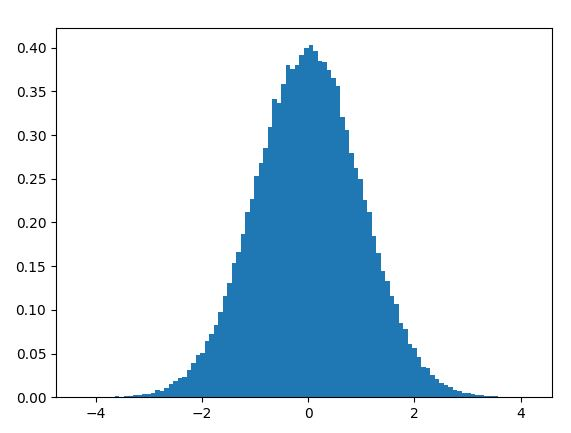
\includegraphics[width=0.7\textwidth]{figures/hist100BinsDensity}
\end{figure}

\vspace*{-5mm}

\begin{itemize}
	\item same histogram, except total area of rectangles is normalized to be $1$
\end{itemize}

\end{frame}


%==============================================================

\begin{frame}[fragile]

\frametitle{Normalized histogram with PDF}

\begin{figure}[ht]
	\centering
	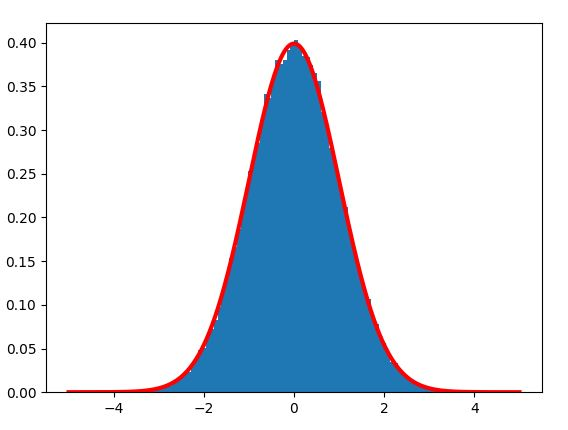
\includegraphics[width=0.7\textwidth]{figures/histWithpdf}
\end{figure}

\vspace*{-5mm}

\begin{itemize}
	\item[] red curve is \red{\emph{probability density function (PDF)}}
\end{itemize}

\end{frame}

%==============================================================

\begin{frame}[fragile]

\frametitle{Probability density functions}

If $X$ is a random number drawn from a distribution with PDF $f(x)$, probability $X$ takes a value in interval $[a,b]$ is
\vspace*{-2mm}
\[
	\boxed{
\mathrm{P}(a \leq X \leq b) = \int_a^b f(x) dx}
\]
\vspace*{-5mm}
\begin{figure}[ht]
	\centering
	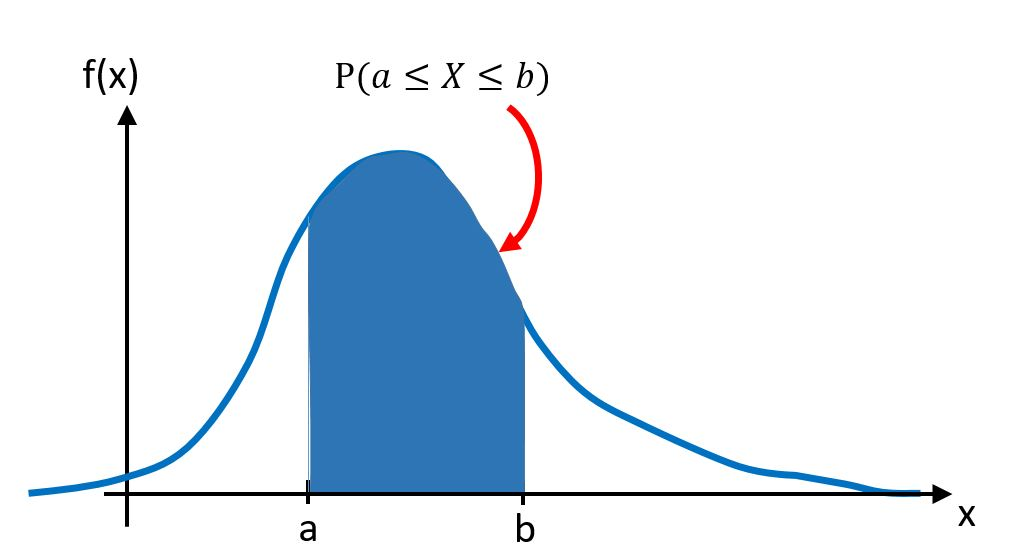
\includegraphics[width=.7\textwidth]{figures/genericPDF}
\end{figure}

\end{frame}

%%==============================================================
%
%\begin{frame}[fragile]
%
%\frametitle{Computing probabilities using standard normal distribution}
%
%\begin{itemize}
%	\item probability of random number $X$ drawn from standard normal distribution taking value in $[a,b]$:
%	\[
%	\mathrm{P}(a \leq X \leq b) = \frac{1}{\sqrt{2\pi}} \int_a^b  e^{-x^2/2} dx
%	\]
%	\item no exact expression exists for $\int_a^b e^{-x^2/2} dx$
%	\begin{itemize}
%		\item need to use numerical integration!
%	\end{itemize}
%\end{itemize}
%
%\end{frame}

%==============================================================

\begin{frame}[fragile]

\frametitle{Example}

Use trapezoidal method to approximate $\mathrm{P}(1 \leq X \leq 2)$ when $X$ is drawn from standard normal distribution
\[
\mathrm{P}(1 \leq X \leq 2) = \frac{1}{\sqrt{2\pi}} \int_1^2 e^{-x^2/2} dx \approx \mathbf{\red{0.1359}}
\]

\vspace*{-5mm}
\begin{figure}[ht]
	\centering
	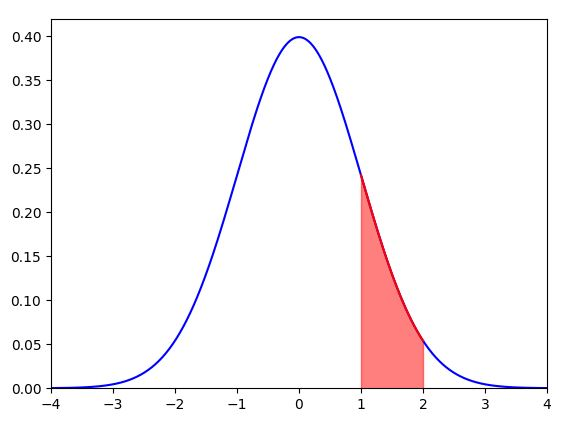
\includegraphics[width=.5\textwidth]{figures/stdnormal_12}
\end{figure}

\end{frame}

%==============================================================

\begin{frame}[fragile]

\frametitle{}

\begin{itemize}
	\item reiterate importance of normal/Gaussian in applications
	\item but standard normal is inflexible
	\item now \textbf{experimentally observe} impact of first two parameters in \texttt{normal()} function call
\end{itemize}

\end{frame}

%==============================================================

\begin{frame}[fragile]

\frametitle{Impact of mean}

\begin{itemize}
	\item shifts average (mean) value
	\item left-right shift of PDF
	\item image here: overlay PDFs for $\mu=0, 5, 20$
\end{itemize}

\end{frame}

%==============================================================

\begin{frame}[fragile]

\frametitle{Mean demo}

\begin{figure}[ht]
	\centering
	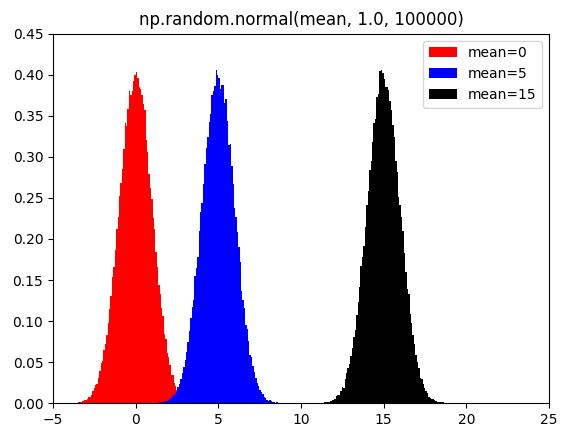
\includegraphics[width=0.7\textwidth]{figures/meanDemoOutput}
\end{figure}

\begin{itemize}
	\item blah
\end{itemize}

\end{frame}

%==============================================================

\begin{frame}[fragile]

\frametitle{Python code}

\texttt{meandemo.py}
\begin{lstlisting}[style=CStyle,basicstyle=\scriptsize]
import numpy as np
import matplotlib.pyplot as plt

def f(x, mu, sigma):
    return 1/(sigma * np.sqrt(2 * np.pi)) * np.exp(-(x - mu)**2 / (2 * sigma**2 ))

x = np.linspace(-5, 30, 1000)

plt.plot(x, f(x, 0, 1), color='r', label='mean=0')
plt.plot(x, f(x, 5, 1), 'b', label='mean=5')
plt.plot(x, f(x, 15, 1), 'k', label='mean=15')
plt.legend()
plt.show()
\end{lstlisting}

\begin{itemize}
	\item blah
\end{itemize}

\end{frame}

%==============================================================

\begin{frame}[fragile]

\frametitle{Impact of standard deviation $\sigma$}

\begin{itemize}
	\item shifts spread of PDF
	\item interpretation of ``standard deviation''
	\item image here
	\item ``most'' of PDF within plus/minus 3 sigma of mean
\end{itemize}

% https://en.wikipedia.org/wiki/Standard_deviation

``In statistics, the standard deviation is a measure of the amount of variation or dispersion of a set of values. A low standard deviation indicates that the values tend to be close to the mean (also called the expected value) of the set, while a high standard deviation indicates that the values are spread out over a wider range.

Standard deviation may be abbreviated SD, and is most commonly represented in mathematical texts and equations by the lower case Greek letter sigma $\sigma$

\end{frame}

%==============================================================

\begin{frame}[fragile]

\frametitle{Impact of stedev}

\begin{itemize}
	\item xxx
\end{itemize}

\end{frame}

%==============================================================

\begin{frame}[fragile]

\frametitle{Stddev demo}

%\begin{figure}[ht]
%	\centering
%	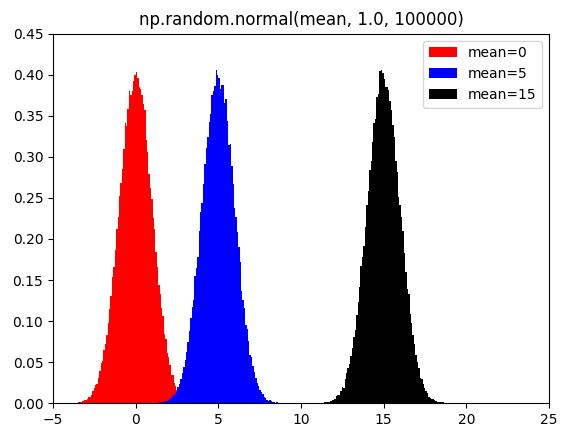
\includegraphics[width=0.7\textwidth]{figures/meanDemoOutput}
%\end{figure}

\begin{itemize}
	\item blah
\end{itemize}

\end{frame}

%==============================================================

\begin{frame}[fragile]

\frametitle{Normal PDF}

\[
\boxed{
	f(x) = \frac{1}{\sigma\sqrt{2\pi}} e^{-\frac{1}{2}\left(\frac{x-\mu}{\sigma}\right)^2}}
\]

\begin{itemize}
	\item mean $\mu$
	\item standard deviation $\sigma$
	\item what are you expected to do with this PDF?
	\begin{enumerate}
		\item call np.random.standard() to generate random numbers for specified $\mu$ and $\sigma$
		\item compute prob X in range $[a,b]$ using numerical integration (trapezoidal)
	\end{enumerate}
\end{itemize}

\end{frame}

%==============================================================

\begin{frame}[fragile]

\frametitle{Standard normal as special case}

Important special case: $\mu=0$ and $\sigma=1$

\[
f(x) = \frac{1}{\sqrt{2\pi}} e^{-\frac{1}{2}x^2}
\]

\textbf{Key point:} standard normal distribution has a mean of $0$ and a standard deviation of $1$

\end{frame}

%==============================================================

\begin{frame}[fragile]

\frametitle{Application 1}

\begin{itemize}
	\item xxx
\end{itemize}

\end{frame}

%==============================================================

\begin{frame}[fragile]

\frametitle{Application 2}

\begin{itemize}
	\item xxx
\end{itemize}

\end{frame}

%==============================================================

\begin{frame}[fragile]

\frametitle{$2)$ Curve-fitting}

\begin{itemize}
	\item straight line fitting
	\item low-order polynomials
	\item maybe fitting exponentials (?)
	\item \texttt{scipy.optimize.curve\_fit}
	\item applications
\end{itemize}

\end{frame}

%==============================================================

\begin{frame}[fragile]

\frametitle{}

\begin{figure}[ht]
	\centering
	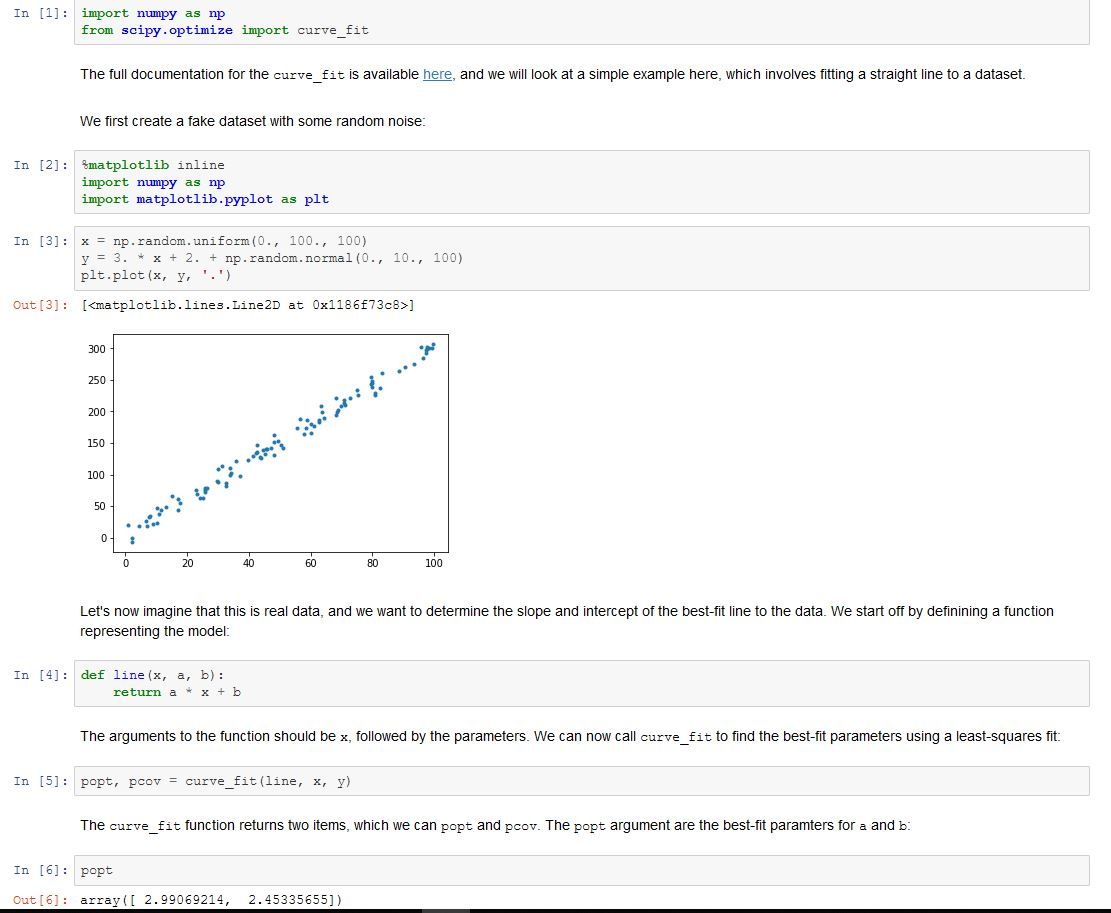
\includegraphics[width=\textwidth]{figures/linearfitscratch}
\end{figure}

% https://astrofrog.github.io/py4sci/_static/15.%20Fitting%20models%20to%20data.html

\begin{itemize}
	\item xxx
\end{itemize}

\end{frame}


%==============================================================

\begin{frame}[fragile]

\frametitle{}

\begin{itemize}
	\item xxx
\end{itemize}

\end{frame}

%==============================================================

\begin{frame}[fragile]

\frametitle{}

\begin{itemize}
	\item xxx
\end{itemize}

\end{frame}

%==============================================================

\begin{frame}[fragile]

\frametitle{}

\begin{itemize}
	\item xxx
\end{itemize}

\end{frame}

%==============================================================

\begin{frame}[fragile]

\frametitle{Lecture summary}
\begin{itemize}
	\item Normal distributions
	\item[]
	
	\item Curve-fitting
	\item[]
	
\end{itemize}

\end{frame}


\end{document}